\documentclass{article}
\usepackage{graphicx} % 
\usepackage{amsmath}%
\usepackage{float}
\graphicspath{{images/}}

\title{\textbf{Power Electronics Laboratory
Session 2: DC-DC converter 2}}
\author{Team 3 : \\Po Ting Yeh K-9056 \\Beyazit Bilal Ozkaya 341967 \\Braulio Cardenas 342021}

\begin{document}
\maketitle
\section*{Introduction}
This experiment explores how a non-ideal synchronous buck converter operates when facing external disturbances. It also introduces a closed-loop control system step by step to improve stability. First, the experiment analyzes the open-loop system's response to load steps and input voltage changes. This shows that the open-loop system cannot adjust automatically and easily loses voltage regulation. Next, an internal inductor current controller is added, which uses a Proportional-Integral (\textbf{PI}) controller and output voltage feedforward. Finally, an external voltage controller is added to create a full cascaded control system. We test this system under strict conditions, including a no-load voltage step and bi-directional power regeneration. The results fully demonstrate the closed-loop system's excellent ability to keep the output voltage stable and reject disturbances.


\section{Part 1: \textbf{Reference Duty Cycle and Signals Measured}}

For these tests a reference duty cycle of $d^* = 0.5$ was chosen. To comprehensively observe the transient behavior, four key signals were measured: the input voltage ($v_{in}$), output voltage ($v_{out}$), inductor current ($i_L$), and output current ($i_{out}$). Monitoring $v_{in}$ is crucial to observe the voltage drop across the input source resistance ($R_s$), while $v_{out}$ indicates the system's regulation capability.
\subsection*{tasks:}
\subsection{Transient Response to Load Step Change}
A load step change was introduced at $t = 0.05\text{s}$ by switching in a parallel resistor, effectively doubling the load demand. As shown in the waveforms, before the disturbance, the system was in a steady state. After $t = 0.05\text{s}$, $i_{out}$ and $i_L$ instantly increased to supply the new load. Consequently, $v_{out}$ experienced a significant drop. Notably, $v_{in}$ also decreased during this transient; this occurs because the higher input current causes a larger voltage drop across the input source resistance ($R_s$).
\\
\begin{figure}[H]
    \centering
    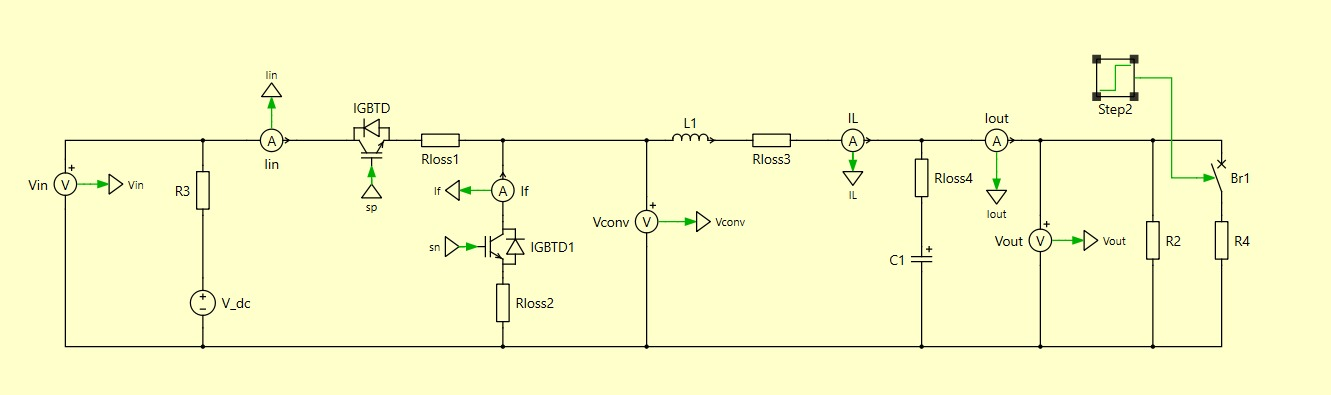
\includegraphics[width=1\linewidth]{images/image2.jpg}
    \caption{Converter circuit schematic}
    \label{fig:placeholder}
\end{figure}
\begin{figure}[H]
    \centering
    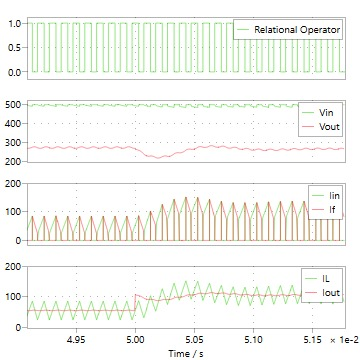
\includegraphics[width=0.75\linewidth]{images/image4.jpg}
    \caption{Load-step transient response}
    \label{fig:placeholder}
\end{figure}

\subsection{Transient Response to DC Input Step Disturbance}
For this test, the ideal input DC source ($V_{dci}$) was stepped down from $500V$ to $450V$ at $t = 0.05\text{s}$. The results show that the output voltage ($v_{out}$) dropped proportionally to the input disturbance. Since this is an open-loop system with a fixed duty cycle, it lacks the ability to adjust the switching signals to reject the input disturbance, resulting in a new, lower steady-state output voltage.
\begin{figure}[H]
    \centering
    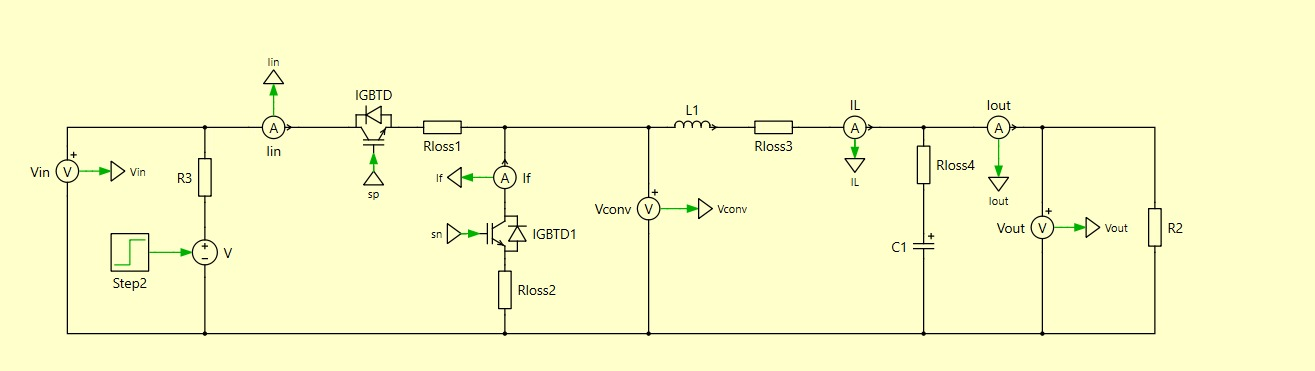
\includegraphics[width=1\linewidth]{images/image7.jpg}
    \caption{Input disturbance circuit}
    \label{fig:placeholder}
\end{figure}
\begin{figure}[H]
    \centering
    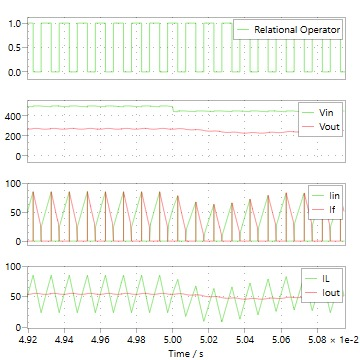
\includegraphics[width=0.75\linewidth]{images/image10.jpg}
    \caption{Input-step transient response}
    \label{fig:placeholder}
\end{figure}
\section{Part 2:}
\subsection*{tasks:}
\begin{figure}[H]
    \centering
    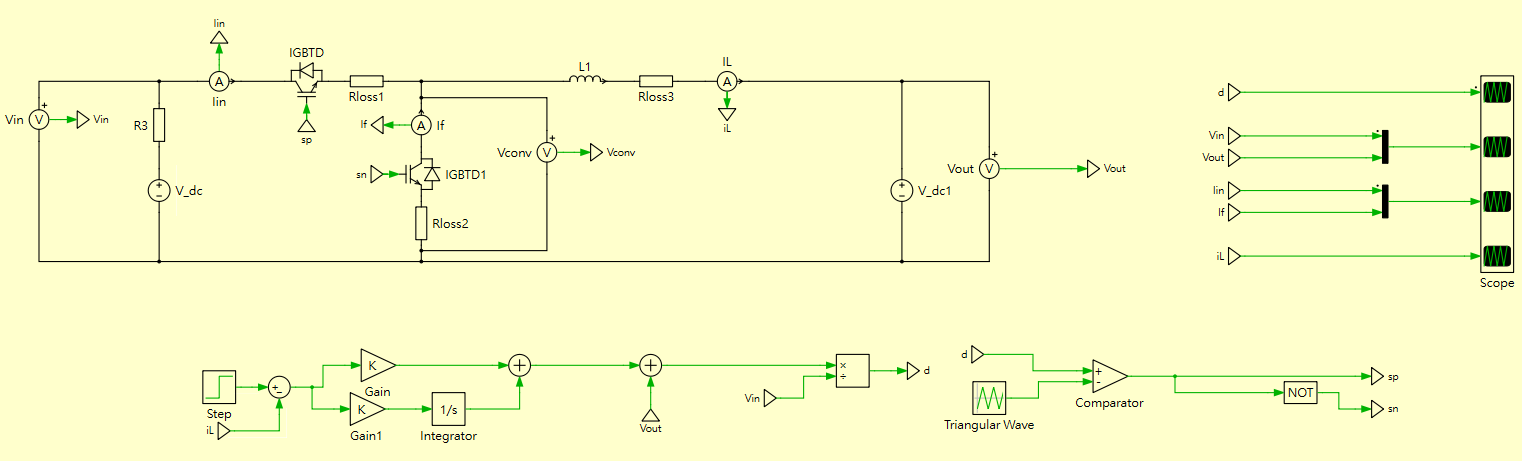
\includegraphics[width=1\linewidth]{images/image5.png}
    \caption{Modified converter schematic}
    \label{fig:placeholder}
\end{figure}
\begin{figure}[H]
    \centering
    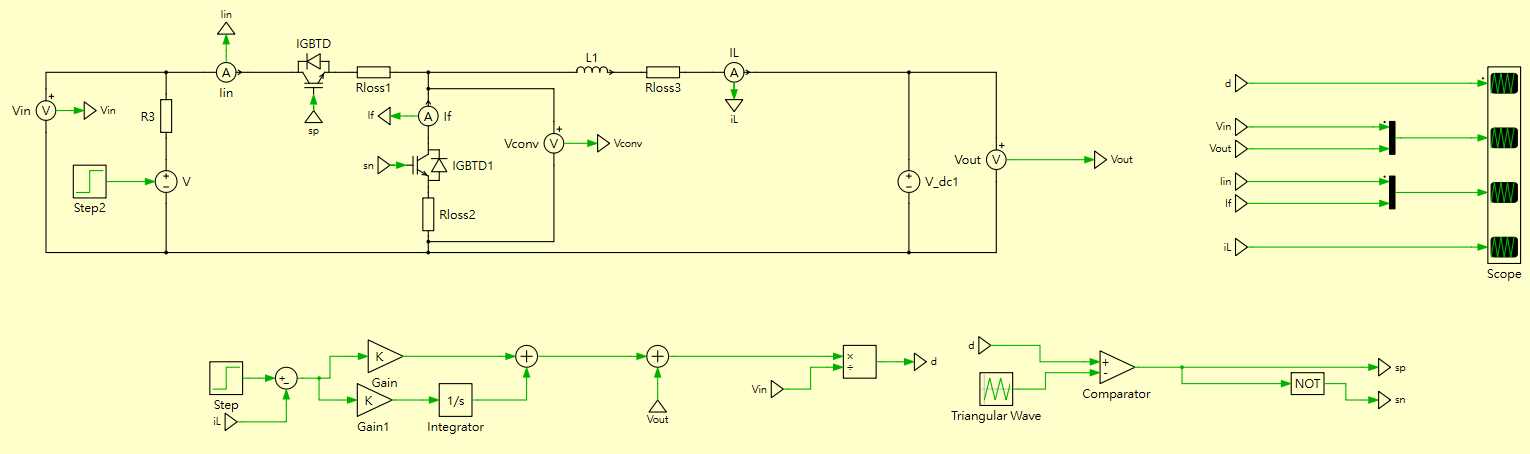
\includegraphics[width=1\linewidth]{images/image11.png}
    \caption{Internal controller implementation}
    \label{fig:placeholder}
\end{figure}
\subsection{Reference current $i_L^* = 0\text{A}$}
\begin{figure}[H]
    \centering
    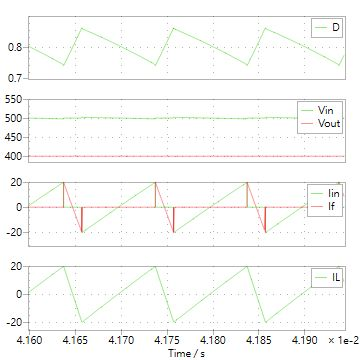
\includegraphics[width=0.75\linewidth]{images/image8.jpg}
    \caption{Current at 0A plots}
    \label{fig:placeholder}
\end{figure}
The internal PI controller successfully regulates the inductor current to track the reference value without steady-state error. Because the output voltage source is set to $V_{dco} = 400\text{V}$ and the input voltage is $V_{in} = 500\text{V}$, the required converter voltage ($v_{conv}$) to maintain a zero-current state is $400\text{V}$. The controller correctly calculates a duty cycle of approximately $D = 400 / 500 = 0.8$ to balance the voltage across the inductor. The current oscillates symmetrically around zero due to the expected switching ripple.

\subsection{Current step from $0\text{A}$ to $10\text{A}$}
\begin{figure}[H]
    \centering
    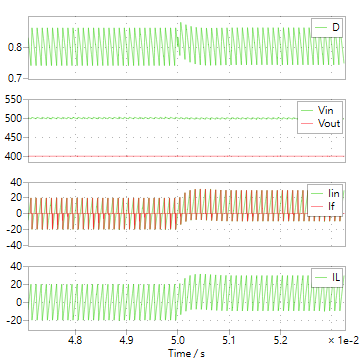
\includegraphics[width=0.75\linewidth]{images/image1.png}
    \caption{Current step to 10A}
    \label{fig:placeholder}
\end{figure}
This demonstrates the excellent transient response of the PI controller. When the step occurs, the proportional gain ($K_{ip}$) responds instantly to the current error, causing the duty cycle to spike. This applies a positive voltage across the inductor ($v_{conv} > v_{out}$), forcing the current to ramp up quickly. Once the current reaches $10\text{A}$, the integral gain ($K_{ii}$) ensures zero steady-state error. The new steady-state duty cycle is slightly higher than the previous $0.8$ because it now needs to compensate for the additional voltage drops across the parasitic resistances ($I \times R_{loss}$) caused by the $10\text{A}$ current flow.

\subsection{Input voltage step disturbance of $10\text{V}$}
\begin{figure}[H]
    \centering
    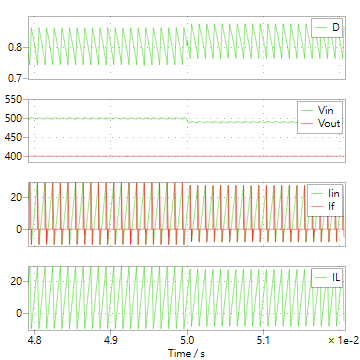
\includegraphics[width=0.75\linewidth]{images/image6.png}
    \caption{10 V input disturbance}
    \label{fig:placeholder}
\end{figure}
This result highlights the critical advantage of the output voltage feedforward and reference scaling (the $1/v_{in}$ block) in the control loop. When the input voltage drops, the scaling block instantaneously recalculates and increases the duty cycle ($D = v_{conv}^* / v_{in}$) to maintain the same actual converter voltage. Because the duty cycle adjusts instantly to the line disturbance, the inductor current just slight decrease. The system effectively rejects the input voltage disturbance before the PI controller even needs to react to a current error.


\section{Part 3: }
\begin{figure}[H]
    \centering
    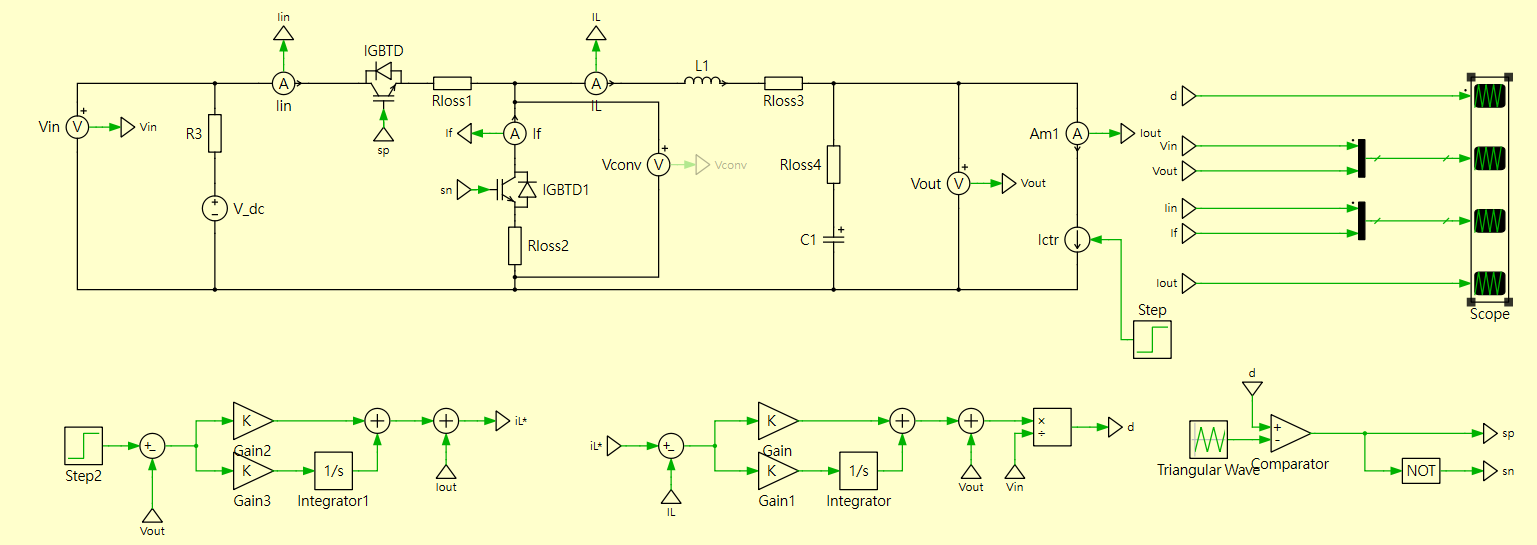
\includegraphics[width=1\linewidth]{images/image3.png}
    \caption{Cascaded control diagram}
    \label{fig:placeholder}
\end{figure}
\subsection*{tasks:}
\subsection{Voltage Reference Step (250V to 400V at No Load)}
\begin{figure}[H]
    \centering
    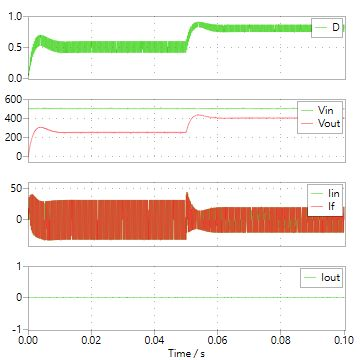
\includegraphics[width=0.75\linewidth]{images/image9.jpg}
    \caption{Voltage reference step}
    \label{fig:placeholder}
\end{figure}
\subsubsection*{Observations:}  The output current ($I_{out}$) remains at 0A as specified. At $t = 0.05$s, the voltage reference steps from 250V to 400V. The output voltage ($V_{out}$) tracks the reference smoothly, rising from 250V to 400V with a well-damped transient response and minimal overshoot. During this transient, a surge in the converter current is observed. The duty cycle ($D$) shifts from approximately 0.5 to 0.8.
\subsubsection*{Comments:} The cascaded control loop operates accurately. The outer voltage PI controller detects the positive voltage error and commands a higher reference current. The inner current controller then temporarily increases the duty cycle to supply the necessary current to charge the output capacitor. Once the capacitor reaches the target voltage of 400V, the current returns to near zero (supplying only no-load losses), and the system settles perfectly into its new steady state.

\subsection{Output Voltage Regulation and Power Regeneration}
\begin{figure}[H]
    \centering
    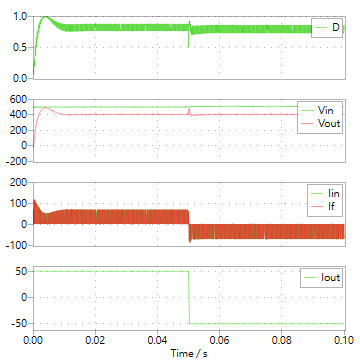
\includegraphics[width=0.75\linewidth]{images/image12.png}
    \caption{Regeneration and regulation}
    \label{fig:placeholder}
\end{figure}
\subsubsection*{Observations:} The output voltage ($V_{out}$) is successfully regulated at 400V. From $t = 0$ to $0.05$s, the load consumes 50A, and the converter currents are positive. At $t = 0.05$s, the load current steps to -50A, entering the regeneration mode. During this transition, $V_{out}$ exhibits an extremely small, well-damped upward spike before settling back exactly to 400V. Simultaneously, the inductor and switch currents immediately reverse their direction to negative values (average -50A). The duty cycle dynamically adjusts to maintain the voltage.
\subsubsection*{Comments:} This result perfectly demonstrates the robust bi-directional capability of the synchronous buck converter and the effectiveness of the cascaded control loop. When the load regenerates power (-50A), it acts as a source pumping charge into the output capacitor. The outer voltage controller and the load current feedforward instantly command a negative reference current. The inner current controller then reduces the duty cycle, forcing the converter to extract the excess energy from the capacitor and feed it backward into the 500V input DC source. This allows the system to seamlessly absorb the regenerated energy while perfectly maintaining the 400V output regulation.

\section*{Conclusions}
Through this experiment, we successfully proved the necessity and advantages of a closed-loop cascaded control system in power converters. In the open-loop tests, the output voltage dropped significantly when the load increased or the input voltage decreased. After adding the internal current controller, the system could track the target current accurately with zero steady-state error. Moreover, the voltage feedforward design instantly canceled out input voltage drops, showing great disturbance rejection. In the final cascaded control system, the external voltage controller and internal current controller worked together perfectly. They achieved smooth voltage tracking from 250V to 400V with very low overshoot. They also showed outstanding dynamic response when the load current switched suddenly between 50A (consuming power) and -50A (regenerating power). The controllers quickly adjusted the duty cycle to send extra energy back to the input, keeping the output voltage perfectly at 400V. Overall, this experiment successfully demonstrated the great performance of cascaded control in bi-directional power transfer and voltage regulation.



\end{document}
